\section{Self-Signed PGP Certificates}

Creating PGP keys was very easy thanks to GPG. The command line tool stepped through each stage very simply. After creating and exporting both the private and public keys for Jason and Toni, display icons were added and then the certificates were uploaded to https://keyserver.pgp.com/. Details of creating the certificate are listed below. 

\noindent Firstly, we used GPG to select the type of key encryption. We opted for the default RSA.
\begin{figure}[hbt!]
	\centering
      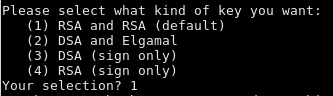
\includegraphics[width=0.5\textwidth]{imgs/pgp/1} \\
	\caption{Selecting key encryption}
	\label{fig:selectkey}
    \noindent\makebox[\linewidth]{}
\end{figure}

\noindent Next we specified the size of the key, again we chose 2048 (default)

\begin{figure}[hbt!]
	\centering
      
\includegraphics[width=0.8\textwidth]{imgs/pgp/2} \\
	\caption{Specifying keysize}
	\label{fig:specifiyingkeysize}
    \noindent\makebox[\linewidth]{}
\end{figure}

\noindent Now we selected how long we would like the key to last. We chose 0, so that the key will not expire)

\begin{figure}[hbt!]
	\centering
      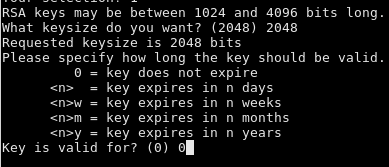
\includegraphics[width=0.5\textwidth]{imgs/pgp/3} \\
	\caption{Specifying how long key will last}
	\label{fig:specifiyingkeysize}
    \noindent\makebox[\linewidth]{}
\end{figure}
\newpage
\noindent GPG now requires information about the key identity, information such as name and email are supplied.)

\begin{figure}[hbt!]
	\centering
      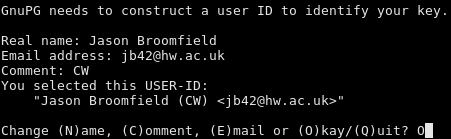
\includegraphics[width=0.6\textwidth]{imgs/pgp/4} \\
	\caption{Filling in key identity information}
	\label{fig:specifiyingkeysize}
    \noindent\makebox[\linewidth]{}
\end{figure}

\noindent After supplying a passphrase for the key, it is added to the local keychain

\begin{figure}[hbt!]
	\centering
      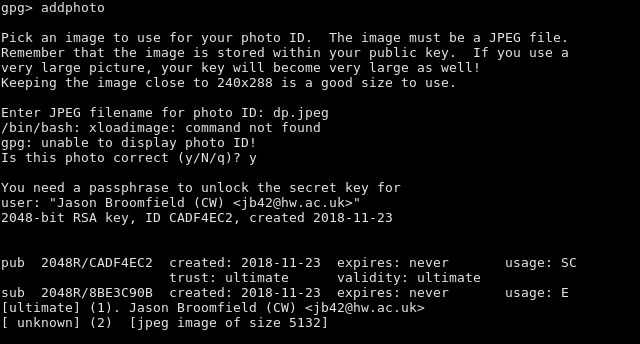
\includegraphics[width=0.6\textwidth]{imgs/pgp/6} \\
	\caption{Defining passphrase and creation}
	\label{fig:specifiyingkeysize}
    \noindent\makebox[\linewidth]{}
\end{figure}

\noindent Keys added to keychain (including Antonio's):

\begin{figure}[hbt!]
	\centering
      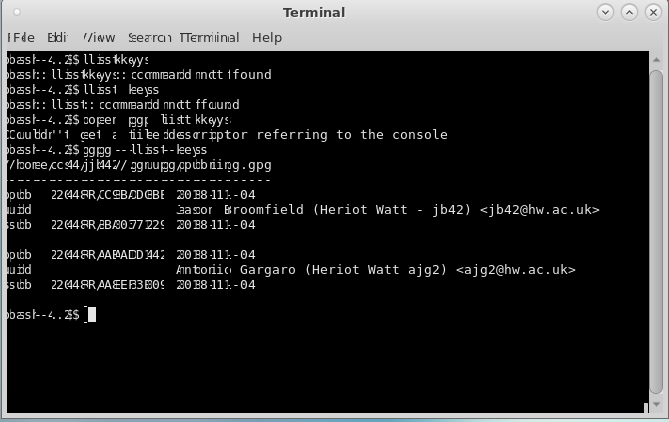
\includegraphics[width=0.6\textwidth]{imgs/pgp/final} \\
	\caption{Keychain}
	\label{fig:specifiyingkeysize}
    \noindent\makebox[\linewidth]{}
\end{figure}

\subsection{Adding display icon to PGP}

\noindent To add icons, we used gpg addphoto on the specified key
\begin{figure}[hbt!]
	\centering
      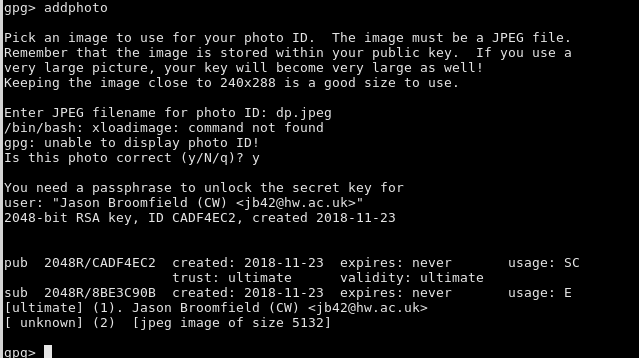
\includegraphics[width=0.6\textwidth]{imgs/pgp/icon} \\
	\caption{Key including display icon}
	\label{fig:specifiyingkeysize}
    \noindent\makebox[\linewidth]{}
\end{figure}

\noindent Finally, we uploaded the key to a server
\begin{figure}[hbt!]
	\centering
      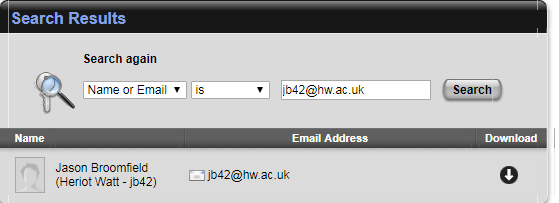
\includegraphics[width=0.6\textwidth]{imgs/pgp/Capture} \\
	\caption{PGP Server}
	\label{fig:specifiyingkeysize}
    \noindent\makebox[\linewidth]{}
\end{figure}


